% -*- Mode:TeX -*-

%% IMPORTANT: The official thesis specifications are available at:
%%            http://libraries.mit.edu/archives/thesis-specs/
%%
%%            Please verify your thesis' formatting and copyright
%%            assignment before submission. If you notice any
%%            discrepancies between these templates and the 
%%            MIT Libraries' specs, please let us know
%%            by e-mailing thesis@mit.edu

%% The documentclass options along with the pagestyle can be used to generate
%% a technical report, a draft copy, or a regular thesis. You may need to
%% re-specify the pagestyle after you \include cover.tex. For more
%% information, see the first few lines of mitthesis.cls. 

%\documentclass[12pt,vi,twoside]{mitthesis}
%%
%%  If you want your thesis copyright to you instead of MIT, use the
%%  ``vi'' option, as above.
%%
%\documentclass[12pt,twoside,leftblank]{mitthesis}
%%
%% If you want blank pages before new chapters to be labelled ``This
%% Page Intentionally Left Blank'', use the ``leftblank'' option, as
%% above. 

\documentclass[12pt,twoside]{mitthesis}
\usepackage{lgrind}
%% These have been added at the request of the MIT Libraries, because
%% some PDF conversions mess up the ligatures.  -LB, 1/22/2014
\usepackage{cmap}
\usepackage[T1]{fontenc}
\pagestyle{plain}
\usepackage{comment}
\usepackage{verbatim}
\makeatletter
\newcommand*{\rom}[1]{\expandafter\@slowromancap\romannumeral #1@}
\makeatother

\textheight=22cm
\textwidth=14.5cm

\usepackage{geometry}
 \geometry{
 a4paper,
 left=30mm,
 top=25mm,
 right=20mm,
 bottom=25mm
 }


 \usepackage{subfigure}
 \usepackage{caption}
\usepackage{subcaption}
\usepackage{amsmath}

\usepackage[utf8]{inputenc}
\usepackage{tikz}
\usetikzlibrary{shapes.geometric, arrows}

\tikzstyle{startstop} = [rectangle, rounded corners, minimum width=3cm, minimum height=1cm,text centered, draw=black, fill=red!30]
\tikzstyle{io} = [trapezium, trapezium left angle=70, trapezium right angle=110, minimum width=3cm, minimum height=1cm, text centered, draw=black, fill=orange!30]
\tikzstyle{process} = [rectangle, minimum width=3cm, minimum height=1cm, text centered, text width=3cm, draw=black, fill=orange!30]
\tikzstyle{decision} = [diamond, minimum width=3cm, minimum height=1cm, text centered, draw=black, fill=green!30]
\tikzstyle{arrow} = [thick,->,>=stealth]
%% This bit allows you to either specify only the files which you wish to
%% process, or `all' to process all files which you \include.
%% Krishna Sethuraman (1990).

%\typein [\files]{Enter file names to process, (chap1,chap2 ...), or `all' to process all files:}
\def\all{all}
\ifx\files\all \typeout{Including all files.} \else %\typeout{Including only \files.} \includeonly{\files} \fi

\begin{document}

% -*-latex-*-
% 
% For questions, comments, concerns or complaints:
% thesis@mit.edu
% 
%
% $Log: cover.tex,v $
% Revision 1.9  2019/08/06 14:18:15  cmalin
% Replaced sample content with non-specific text.
%
% Revision 1.8  2008/05/13 15:02:15  jdreed
% Degree month is June, not May.  Added note about prevdegrees.
% Arthur Smith's title updated
%
% Revision 1.7  2001/02/08 18:53:16  boojum
% changed some \newpages to \cleardoublepages
%
% Revision 1.6  1999/10/21 14:49:31  boojum
% changed comment referring to documentstyle
%
% Revision 1.5  1999/10/21 14:39:04  boojum
% *** empty log message ***
%
% Revision 1.4  1997/04/18  17:54:10  othomas
% added page numbers on abstract and cover, and made 1 abstract
% page the default rather than 2.  (anne hunter tells me this
% is the new institute standard.)
%
% Revision 1.4  1997/04/18  17:54:10  othomas
% added page numbers on abstract and cover, and made 1 abstract
% page the default rather than 2.  (anne hunter tells me this
% is the new institute standard.)
%
% Revision 1.3  93/05/17  17:06:29  starflt
% Added acknowledgements section (suggested by tompalka)
% 
% Revision 1.2  92/04/22  13:13:13  epeisach
% Fixes for 1991 course 6 requirements
% Phrase "and to grant others the right to do so" has been added to 
% permission clause
% Second copy of abstract is not counted as separate pages so numbering works
% out
% 
% Revision 1.1  92/04/22  13:08:20  epeisach

% NOTE:
% These templates make an effort to conform to the MIT Thesis specifications,
% however the specifications can change. We recommend that you verify the
% layout of your title page with your thesis advisor and/or the MIT 
% Libraries before printing your final copy.
\title{MIT Thesis Template in Overleaf}

\author{Tim Beaver}
% If you wish to list your previous degrees on the cover page, use the 
% previous degrees command:
%       \prevdegrees{A.A., Harvard University (1985)}
% You can use the \\ command to list multiple previous degrees
%       \prevdegrees{B.S., University of California (1978) \\
%                    S.M., Massachusetts Institute of Technology (1981)}
\department{Department of Electrical Engineering and Computer Science}

% If the thesis is for two degrees simultaneously, list them both
% separated by \and like this:
% \degree{Doctor of Philosophy \and Master of Science}
\degree{Bachelor of Science in Computer Science and Engineering}

% As of the 2007-08 academic year, valid degree months are September, 
% February, or June.  The default is June.
\degreemonth{June}
\degreeyear{1990}
\thesisdate{May 18, 1990}

%% By default, the thesis will be copyrighted to MIT.  If you need to copyright
%% the thesis to yourself, just specify the `vi' documentclass option.  If for
%% some reason you want to exactly specify the copyright notice text, you can
%% use the \copyrightnoticetext command.  
%\copyrightnoticetext{\copyright IBM, 1990.  Do not open till Xmas.}

% If there is more than one supervisor, use the \supervisor command
% once for each.
\supervisor{William J. Supervisor}{Associate Professor}

% This is the department committee chairman, not the thesis committee
% chairman.  You should replace this with your Department's Committee
% Chairman.
\chairman{Arthur C. Chairman}{Chairman, Department Committee on Graduate Theses}

% Make the titlepage based on the above information.  If you need
% something special and can't use the standard form, you can specify
% the exact text of the titlepage yourself.  Put it in a titlepage
% environment and leave blank lines where you want vertical space.
% The spaces will be adjusted to fill the entire page.  The dotted
% lines for the signatures are made with the \signature command.
\maketitle

% The abstractpage environment sets up everything on the page except
% the text itself.  The title and other header material are put at the
% top of the page, and the supervisors are listed at the bottom.  A
% new page is begun both before and after.  Of course, an abstract may
% be more than one page itself.  If you need more control over the
% format of the page, you can use the abstract environment, which puts
% the word "Abstract" at the beginning and single spaces its text.

%% You can either \input (*not* \include) your abstract file, or you can put
%% the text of the abstract directly between the \begin{abstractpage} and
%% \end{abstractpage} commands.

% First copy: start a new page, and save the page number.
\cleardoublepage
% Uncomment the next line if you do NOT want a page number on your
% abstract and acknowledgments pages.
% \pagestyle{empty}
\setcounter{savepage}{\thepage}
\begin{abstractpage}
% $Log: abstract.tex,v $
% Revision 1.1  93/05/14  14:56:25  starflt
% Initial revision
% 
% Revision 1.1  90/05/04  10:41:01  lwvanels
% Initial revision
% 
%
%% The text of your abstract and nothing else (other than comments) goes here.
%% It will be single-spaced and the rest of the text that is supposed to go on
%% the abstract page will be generated by the abstractpage environment.  This
%% file should be \input (not \include 'd) from cover.tex.
Lorem ipsum dolor sit amet, consectetur adipiscing elit. Nam quis neque et erat laoreet finibus at ac leo. Curabitur pellentesque, diam quis dignissim finibus, enim dui feugiat leo, nec porttitor sapien mi ac felis. Nam aliquam pretium nibh, quis dapibus dolor gravida sit amet. Cras porttitor dui quis elementum pulvinar. Nulla id pulvinar massa. Nullam ut diam non lorem venenatis faucibus. Vivamus lacus ante, pellentesque vitae nisl sit amet, bibendum facilisis purus.

\end{abstractpage}

% Additional copy: start a new page, and reset the page number.  This way,
% the second copy of the abstract is not counted as separate pages.
% Uncomment the next 6 lines if you need two copies of the abstract
% page.
% \setcounter{page}{\thesavepage}
% \begin{abstractpage}
% % $Log: abstract.tex,v $
% Revision 1.1  93/05/14  14:56:25  starflt
% Initial revision
% 
% Revision 1.1  90/05/04  10:41:01  lwvanels
% Initial revision
% 
%
%% The text of your abstract and nothing else (other than comments) goes here.
%% It will be single-spaced and the rest of the text that is supposed to go on
%% the abstract page will be generated by the abstractpage environment.  This
%% file should be \input (not \include 'd) from cover.tex.
Lorem ipsum dolor sit amet, consectetur adipiscing elit. Nam quis neque et erat laoreet finibus at ac leo. Curabitur pellentesque, diam quis dignissim finibus, enim dui feugiat leo, nec porttitor sapien mi ac felis. Nam aliquam pretium nibh, quis dapibus dolor gravida sit amet. Cras porttitor dui quis elementum pulvinar. Nulla id pulvinar massa. Nullam ut diam non lorem venenatis faucibus. Vivamus lacus ante, pellentesque vitae nisl sit amet, bibendum facilisis purus.

% \end{abstractpage}

\cleardoublepage

\section*{Acknowledgments}

This is the acknowledgements section. You should replace this with your
own acknowledgements.

%%%%%%%%%%%%%%%%%%%%%%%%%%%%%%%%%%%%%%%%%%%%%%%%%%%%%%%%%%%%%%%%%%%%%%
% -*-latex-*-

% Some departments (e.g. 5) require an additional signature page.  See
% signature.tex for more information and uncomment the following line if
% applicable.
% % -*- Mode:TeX -*-
%
% Some departments (e.g. Chemistry) require an additional cover page
% with signatures of the thesis committee.  Please check with your
% thesis advisor or other appropriate person to determine if such a 
% page is required for your thesis.  
%
% If you choose not to use the "titlepage" environment, a \newpage
% commands, and several \vspace{\fill} commands may be necessary to
% achieve the required spacing.  The \signature command is defined in
% the "mitthesis" class
%
% The following sample appears courtesy of Ben Kaduk <kaduk@mit.edu> and
% was used in his June 2012 doctoral thesis in Chemistry. 

\begin{titlepage}
\begin{large}
This doctoral thesis has been examined by a Committee of the Department
of Chemistry as follows:

\signature{Professor Jianshu Cao}{Chairman, Thesis Committee \\
   Professor of Chemistry}

\signature{Professor Troy Van Voorhis}{Thesis Supervisor \\
   Associate Professor of Chemistry}

\signature{Professor Robert W. Field}{Member, Thesis Committee \\
   Haslam and Dewey Professor of Chemistry}
\end{large}
\end{titlepage}


\pagestyle{plain}
  % -*- Mode:TeX -*-
%% This file simply contains the commands that actually generate the table of
%% contents and lists of figures and tables.  You can omit any or all of
%% these files by simply taking out the appropriate command.  For more
%% information on these files, see appendix C.3.3 of the LaTeX manual. 
\tableofcontents
\newpage
\listoffigures
\newpage
\listoftables


%% This is an example first chapter.  You should put chapter/appendix that you
%% write into a separate file, and add a line \include{yourfilename} to
%% main.tex, where `yourfilename.tex' is the name of the chapter/appendix file.
%% You can process specific files by typing their names in at the 
%% \files=
%% prompt when you run the file main.tex through LaTeX.
\chapter{An Introduction to our Dark Universe}

\section{Introduction}
"Our whole universe was in a hot dense state,
then nearly fourteen billion years ago expansion started..."Every time I listen to the song from the hot drama "the big bang theory", it make me recall my fascination about the process that our universe went through with a bunch of miracle, and in the end, I can sit here and write the thesis for my master degree. At the starting, there is just a very hot, dense initial state stationing in our universe, Suddenly, it blows off in an extremely short time. In finale, the abundant light elements, the cosmological microwave background(CMB) as well as the large-scale structure are presented in our universe.\\

From the modern astrophysical point of view, our universe consists of three parts of the things, including the material, the dark matter. and also the dark energy. Unfortunately, now we only get the material acknowledged. Basically, we only understand about 4\% of our universe! How to unveil the mystery of the dark matter is now the most popular topic around the world.\\

In this chapter, I will first give a brief introduction about the history of cosmological model of our universe, leading to two "missing mysteries", encompassing "missing energy(dark energy)" and "missing mass(dark matter)". Then, some of the evidence from astrophysics on the dark matter will be performed. \\


\include{chap2}
%% This is an example first chapter.  You should put chapter/appendix that you
%% write into a separate file, and add a line \include{yourfilename} to
%% main.tex, where `yourfilename.tex' is the name of the chapter/appendix file.
%% You can process specific files by typing their names in at the 
%% \files=
%% prompt when you run the file main.tex through LaTeX.
\chapter{Introduction for TEXONO experiments}

\section{Data Preparation: L/M shells X-ray subtraction}
After the raw data is obtained with some primary calibrations, the next step will be the subtraction of the K/L shells X-ray contributions. Since several characteristic K shell X-ray peaks from internal cosmogenic radioactive isotopes can be recognized in the data, and the ratios of the K-shell to L-shell X-ray events, which is well-predicted with the great agreement of the measurement as written in Ref. [12], can be employed to get the intensity of the L-shell X-rays in the lower energy ranges (<1.6 keVee). The process is as follows:
\begin{enumerate}
	\item In Figure\ref{}, the peaks for five isotopes, including $Ge^{68}$, $Ga^{68}$, $Zn^{65}$, $Fe^{55}$, $V^{49}$, can be identified clearly with some of the gaussian fits. \\
	
        \begin{figure}[h]
        \includegraphics[scale=0.6]{/Users/yehchihhsiang/Desktop/Analysis/CDEX_Analysis_method/Codes/Thesis_Plot/MLshells_Subtraction/Resolution_Plot1.pdf}
        \centering
        \caption{The process of an interaction for a WIMP with an atom.} \label{Interaction}
        \end{figure}
        
	\item In the paper\ref{}, the ratios of the K-shell to L-shell X-ray events are well-measured.  As the event number is calculated by the integral of the gaussians, the following formula is used in the calculation:\\
	\begin{equation}
        \label{Gaussian Area}
        Area  = a \times c \times \sqrt{2 \pi} 
        \end{equation}
        a is the constant of the gaussian, and c is the uncertainty of the gaussian.
        	\item With the number of the transformation, the event number from L shells can be inferred by the scaling factor given in the \ref{}. In the end, the gaussian can be fitted at the energies of L shells with the known event numbers. In Figure\ref{}, the gaussians for five isotopes can be recognized. In the end, the subtraction can be completed, as the pink points drawn in the plot. \\
        \begin{figure}[h]
        \includegraphics[scale=0.6]{/Users/yehchihhsiang/Desktop/Analysis/CDEX_Analysis_method/Codes/Thesis_Plot/MLshells_Subtraction/Resolution_Plot2.pdf}
        \centering
        \caption{The process of an interaction for a WIMP with an atom.} \label{Interaction}
        \end{figure}

\section{Earth Attenuation Model}
Because of the environment, which incloses the detector, can let WIMPs loss the energies on their ways to the detector, furthermore, when the energies of WIMPs are lower than the triggering energy of the detector, the experiment would not be allowed to explore WIMPs above the critical energy loss, at this particular point, the densities for the material of the environment should be well-recognized for calculating the energy loss of WIMPs exactly. Three models, which are utilized in our analysis, are described as follows:

\begin{enumerate}
	\item Inner-Earth Model: Based on the research of using P and S waves to predict the densities of the inner-earth structure, the "Preliminary Reference Earth Model"(PREM) is established as written in the reference\cite{}.  In Fig.\ref{}, it visualizes the densities of the inner-earth structure applied to our analysis. 
	\item Atmospheric Model: Based on the theoretical calculation, "The 1976 U.S. Standard Atmosphere"\cite{}, which is the most popular model for describing the atmosphere, is adopted as our atmospheric model as visualized in Fig.\ref{}.
	\item Shielding Model: Two parts of the shielding that are taken into account. The first part is the passive shielding layers, that are 5 cm of copper, 25 cm of boron-loaded polyethylene, 5 cm of steel, and 15 cm of lead consecutively from inside out. Another part is the structure of the building around the detector. In our analysis, 1 m of wall, 10 m of ceiling (30 meter-water-equivalent thickness), and the reactor with 28 m radius nearby the detector are consider precisely. 

\end{enumerate}


%% This is an example first chapter.  You should put chapter/appendix that you
%% write into a separate file, and add a line \include{yourfilename} to
%% main.tex, where `yourfilename.tex' is the name of the chapter/appendix file.
%% You can process specific files by typing their names in at the 
%% \files=
%% prompt when you run the file main.tex through LaTeX.

\chapter{Analysis Strategies}
%%%%%%%%%%%%%%%%%%%%%%%%%%%%%%%%%%%%%%%%%%%%%%%%%%%%%%%%%%%%%%%%%%%%%%%%%%%%%%%%%
\section{Introduction}
In our studies, the major aim is to figure out that after a bunch of WIMPs come over to our detector through various layers of solid earth, air and shielding with the disparate densities, which are claimed by our earth, air model as well as the structure of the shielding surrounding by the germanium detector in the previous sections, how many WIMPs can still survive and retain energized to give our detector "multiple hits" after lots of "barricades" stationing on their way to the detector.\\

In the first place, since some of the terminologies are applied throughout our studies frequently, in the first section, two subsets of definitions, including vacuum/ earth effect cases, as well as the modes of WIMPs flying to our detector, would be well-written. Then, as the crux process of all fashions, which are detailed in the inferior sections, "an interaction" between the atom and the WIMP should be equipped in advance. Later on, three interacting channels, which are employed to make the measurement on WIMPs realized, are depicted as the highlight of our studies in the following section. In the end, speaking of setting limits on WIMPs, the exclusion plot, which is the battleground for all direct-detection experiments on detecting WIMPs, must be conceptualized ahead of time, then the vacuum-constrained cases are delivered as the specifications for the preparation of taking the earth effect into account.

%%%%%%%%%%%%%%%%%%%%%%%%%%%%%%%%%%%%%%%%%%%%%%%%%%%%%%%%%%%%%%%%%%%%%%%%%%%%%%%%%
\section{Definition Clarifications}
\subsection{Vacuum Case\&Earth Effect Case}
There are two types of cases that should be defined as the consensus for our studies:
\begin{enumerate}
	\item Vacuum case:\\
	 Vacuum, which means "devoid of matter in the space", is an analogy in our studies, indicates that the intensity of interaction between WIMPs and atoms is too low, resulting in all material on the route WIMPs traverse to the detector seems transparent to WIMPs. In other words, any material can't make them decelerated supposedly. The interactions with the material are { \bf totally overlooked}, except their interactions with our detector.
	\item Earth Effect Case:\\
	In contrast to the vacuum case, the interactions between WIMPs and atoms, comprising the material of solid earth, air, and shielding, are taken into account precisely. 
\end{enumerate}

\subsection{Trajectory for WIMPs: S-mode\&B-mode}
In our research, two modes for simulating the flying WIMPs from our universe are as follows:
\begin{enumerate}
	\item S-mode:\\
	The trajectory of the S-mode is a straight line. Under this mode, all of the WIMPs in our universe fly directly to our detector with a straight line defaultly. The scheme for this mode is in Fig.\ref{}.
	\item B-mode:\\
	The trajectory of the B-mode is a bending line. Under this mode, WIMPs could be bent by the atoms when they come to our detector. The chart for this mode is in Fig.\ref{}.
\end{enumerate}


\section{Core: The loop for An Interaction}
Since the earth effect should be quantified by premeditating the effect of deceleration on the moving WIMPs, the basic interacting process should be demonstrated.\\

In Figure \ref{Interaction}, the process of an interaction between a WIMP and an atom is performed. Having known velocity and mass given at the start for WIMP, the energy loss can be obtained randomly based on the spectrum of $\frac{d\sigma}{dT}$, portraying which energy loss should be opted, according to the cross-section, which is referred to the possibility. In the end, after the energy loss is taken into account, the final velocity and energy of WIMP can be gained.\\

All of the means made use of in our research stick with "an interaction", which is the basic unit erected as the kernel of the mediums since WIMPs can transport an amount of energy to atoms of "solid earth, air, and shielding" through numerous interactions, and this unit plays an important role throughout the entire studies. \\

\begin{figure}
\begin{center}
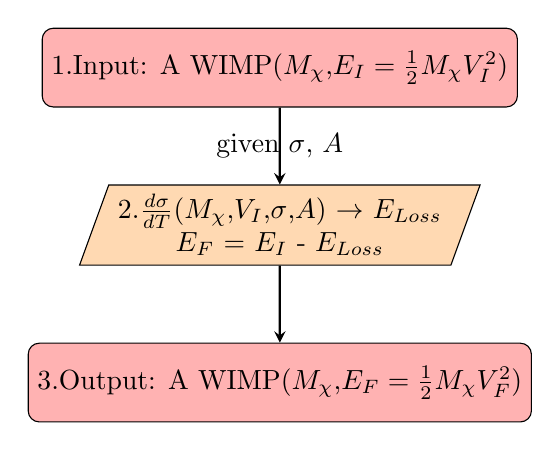
\begin{tikzpicture}[node distance=2cm]
\centering
\node (start) [startstop, align=center] {1.Input: A WIMP($M_{\chi}$,$E_{I}=\frac{1}{2}M_{\chi}V_{I}^{2}$)};
\node (in1) [io, below of=start, align=center] {2.$\frac{d\sigma}{dT}$($M_{\chi}$,$V_{I}$,$\sigma$,$A$) $\rightarrow$ $E_{Loss}$ \\ $E_{F}$ = $E_{I}$ - $E_{Loss}$  };
\node (end) [startstop, below of=in1, align=center] {3.Output: A WIMP($M_{\chi}$,$E_{F}=\frac{1}{2}M_{\chi}V_{F}^{2}$)};


\draw [arrow] (start) -- node{given $\sigma$, $A$}(in1);
\draw [arrow] (in1) -- node{}(end);
\end{tikzpicture}
\end{center}
\caption{The process of an interaction for a WIMP with an atom.} \label{Interaction}
\end{figure}


\section{Three Types of Interacting channels in the Detector}
Because the various channels of interaction are sensitive to the different $M_{\chi}$ with the different cross-sections, comprehending the mechanisms of those channels, and authentically figuring out the rates of WIMPs by those should be well-found. In this section, to begin with, the WIMP-nucleus elastic scattering($\chi-N$ Scattering), which is the typical mechanism for detecting WIMPs, would be reviewed with the fundamental deduction for it. Based on the $\chi-N$ Scattering, two genres of the signal originating from electrons and photons by mechanisms of Migdal Effect and Bremsstrahlung individually were proposed to probe the low-mass WIMPs by some of the theoretical research recently. Therefore, Both of the mechanisms are also taken into consideration as two channels to probe WIMPs, and will be reviewed in this section as well. Hopefully, with the help of these two channels, the low-mass WIMPs with the unexplored cross-sections can be unveiled.

\subsection{$\chi-N$ Scattering}
Traditionally, the atomic electrons around the nucleus of the target material is assumed to have the same motion as the recoil nucleus, meaning that electrons and recoil nucleus are considered as a whole to interact with WIMPs. After the whole Ge is scattered by WIMPs, an amount of energy from WIMPs will be deposited in it. In order to formulate the differential event rate of $\chi-N$ Scattering for the signal of spin-independent WIMPs, the following deduction is utilized in our analysis.

In the first place, the differential WIMP-nucleon cross section can be obtained by the following formula:
\begin{equation}
\frac{d\sigma_{WN}(q)}{dq^{2}} = \frac{\sigma_{0WN}F^{2}(q)}{4\mu_{A}^{2}v^{2}}
\end{equation}
where $\sigma_{0WN}$ is the zero-momentum WIMP-nucleon cross section, $v$ is the velocity of the WIMP in the lab frame, $\mu_{A} \equiv \frac{M_{A}M_{\chi}}{M_{A}+M_{\chi}}$ is the reduced mass of the WIMP-nucleus system, $q$ is the momentum transfer, and $F$ is the nuclear form factor, depending on the model. The Woods-Saxon form factor is suggested to be the good approximation for the spin-independent WIMP, which is suitable for our case:
\begin{equation}
F(q) = \frac{3[\text{sin}(qr_{n})-qr_{n}\text{cos}(qr_{n})]}{(qr_{n})^{3}}e^{\frac{-(qs)^{2}}{2}}
\end{equation}
where 
\begin{equation}
r_{n}^{2} = (1.23A^{1/3}-0.60 \text{fm})^2 + \frac{7}{3}(0.52\pi \text{fm})^{2}-5s^{2}
\end{equation}
$s=0.9$fm, $A$ is the atomic mass of the target, and 
\begin{equation}
q=\sqrt{2M_{A}E_{R}}
\end{equation}
Here, $M_{A}$ is the mass of the target, and $E_{R}$ is the recoil energy.
As the material of the target applied in the different experiments is varying, the dependence of $\sigma_{0WN}$ on the material of the target must be factored out with the new form:
\begin{equation}
\sigma_{0WN,SI} = \sigma_{SI} \frac{\mu_{A}^{2}}{\mu_{n}^{2}} A^{2}
\end{equation}
where
\begin{equation}
\mu_{n} \equiv \frac{M_{n}M_{\chi}}{M_{n}+M_{\chi}}$
\end{equation}

When the differential WIMP-nucleon cross section is built up, the differential cross-section, which will be used in calculating the differential event rate, can be figured out:
\begin{equation}
\frac{d\sigma_{WN}(q)}{dq^{2}} \times 2A = \frac{d\sigma_{WN}(q)}{dq} = \frac{d\sigma_{WN}(q)}{dT} = \frac{d\sigma}{dE_{R}}
\end{equation}

In the end, the differential event rate can be calculated as follows:
\begin{equation}
\frac{dR}{dE_{R}} = N_{T} \frac{\rho_{\chi}}{m_{\chi}}} \int d^{3}\vec{v}vf_{v}(\vec{v}+\vec{v_{E}})\frac{d\sigma}{dE_{R}}
\end{equation}

\subsection{Migdal Effect}
In reality, since the electrons surrounding by the nucleus should take some time to catch up the motion of the nucleus, leading to the effects of ionization and excitation, the signal of the electrons, which can't be generated by the $\chi-N$ scattering, can be acquired for exploring the lower $M_{\chi}$. Being similar to the one adopted in the $\chi-N$ scattering, the differential event rate for the Migdal effect can be expressed as follows:
\begin{equation}
\frac{d^{2}R}{dE_{EM}E_{R}} = N_{T} \frac{\rho_{\chi}}{m_{\chi}}} \int d^{3}\vec{v}vf_{v}(\vec{v}+\vec{v_{E}})\frac{d^{2}\sigma}{dE_{EM}dE_{R}}
\end{equation}
where
\begin{equation}
\frac{d^{2}\sigma}{dE_{EM}E_{R}} = \frac{d\sigma}{dE_{R}} \frac{1}{2\pi}\Sigma_{n,l}\frac{d}{dE_{EM}}p^{c}_{qe}(nl \rightarrow (E_{EM} - E_{nl} ))}
\end{equation}

\subsection{Bremsstrahlung}

$\frac{d^{2}\sigma}{dE_{\gamma}E_{R}} = \frac{4\alpha}{3\pi E_{\gamma}} \frac{E_{R}}{m_{N}c^{2}} |f(E_{\gamma}) |^{2} \times \frac{d\sigma}{dE_{R}} \Theta (E_{\gamma,max}-E_{\gamma})

$f(E_{\gamma}) = f_{1}(E_{\gamma})+if_{2}(E_{\gamma})$

$\frac{d^{2}R}{dE_{\gamma}E_{R}} = N_{T} \frac{\rho_{\chi}}{m_{\chi}}} \int d^{3}\vec{v}vf_{v}(\vec{v}+\vec{v_{E}})\frac{d^{2}\sigma}{dE_{\gamma}dE_{R}}$

%%%%%%%%%%%%%%%%%%%%%%%%%%%%%%%%%%%%%%%%%%%%%%%%%%%%%%%%%%%%%%%%%%%%%%%%%%%%%%%%%
\section{Battleground for WIMPs: Exclusion Plot}
The territory on the map of $\sigma_{SI}$ and $M_{\chi}$, which is also named as "exclusion plot", is adopted to compare the capabilities between a variety of the experiments. The more territory the experiment can advocate, the higher the possibility that it can discover the WIMP, on the other hand, if there is no excess signal from the experiment, it can exclude more regions and encourages other developing experiments to elongate their aptness toward proclaiming more unknown territory. In Fig.\ref{}, the territories claimed by other experiments before are demonstrated. There are three pieces of information that can be acquired from each enclosing region:\\
\begin{enumerate}
\item  Upper boundary: Associated with the location of the detector incorporating with the surrounding shielding.  
\item  Left boundary: The threshold of the detector, relying on the interacting channel considered at the moment.
\item  Lower boundary: Related to the "data-taking period $\times$ the mass of the detector".
\end{enumerate}
From this plot, another intriguing phenomenon is that, if the same territory is asserted by two or more experiments, and one of them assures there is no excess signal popping up from their observation, then it's a cross-check on the findings for each other. Because sometimes, one of them could find out the excess signal within the region which is already excluded by other experiments, then there could be something that is not pondered in the studies, leading to the fake signal, such as electronic noise, the dust on the detector, and so on.\\

In the following studies, since the capabilities of our experiments including TEXONO and CDEX should antagonize with other experiments, the same plot would be utilized as the constraint on WIMPs is accomplished with the certain way under the different conditions.\\

In parallel, because of the gargantuan room for the low-mass region to be investigated with the more lower threshold of the detector, the studies on comprehending the fundamental solid-state physics emerging in the crystal with regard to a stack of parameters, including temperature, impurity level, etc. are terminated. Along with that, the method of amplifying the signal of WIMP directly is also probed for opening another possibility for the discovery of the WIMP. The extension of the studies would be summarized in the section of the "extension studies". 

\section{Vacuum-constrained limits on WIMPs}
Before hunting for the constraint on WIMPs with the earth effect, the vacuum case, meaning that there is no earth effect on WIMPs, should be explored as our criteria, and the numbers of cross-sections captured from this section are considered to be the most considerable preparatory.\\  
\subsection{Concept of Setting limits with Data}
As the model and the data involve divergent information:\\
\begin{enumerate}
\item  Data: "Unknown Physics" + "Known Physics"
\item  Model: "Unknown Physics"
\end{enumerate}
The philosophy of setting limits on WIMPs is that, since the data encompasses more information theoretically, the event number from the assumed models, including those three channels delineated before, can't surpass the data. In our studies, as the form of the event is "rate of WIMP", the spectrum of the rates from the theoretical predictions for WIMPs can't surpass the spectrum obtained from our data. On the other hand, if the rates of the WIMPs from those channels are higher than the ones gotten from the data, the models should be excluded for the unreasonable expectation.\\

Because of the higher rate of WIMP from any of the interacting channel in the detector with respect to the higher cross-section, any model of WIMP can initiate being precluded with the critical cross-section that causes the certain point of modeling spectrum to intersect with the certain upper bound of the point, which corresponds to the 90\% confidence level, derived from the binned Possion method, in the data.

\subsection{Exemplars for cases}
 In Figure\ref{Vacuum-constrained WIMPs}, the data is presented with two Migdal-effect spectrums at masses equal to 1GeV as well as 0.05GeV. As a result of the unearthing of the critical cross-sections, which correspond to the 90\% upper limits confidence level as listed in the figure, the limits set by vacuum are concluded for both masses. When the cross-sections are higher than the critical ones, the spectrums of models will outpace the measured one, which should be entirely excluded as they contradict the core tenet composed before. \\ 
    \begin{figure}[h]
    \includegraphics[scale=0.5]{/Users/yehchihhsiang/Desktop/Analysis/CDEX_Analysis_method/Codes/Thesis_Plot/Lower_Limit_Plot.png}
    \centering
    \caption{The measured spectrum for our analysis (black point), with L/M-shell x-ray contributions from the cosmogenic nuclides in the germanium crystal subtracted. The bin width is 50eVee, and the energy range is 0.16–2.16keVee. The blue dash-dotted line and red dash line are the expected χ-N spectra due to Migdal effect at mχ equal to 50  and 1.0  , at cross-section corresponding to the upper limit at 90\% confidence level, derived by the binned Poisson method.} \label{Vacuum-constrained WIMPs}
    \end{figure}
  
After all of the critical cross-sections are sought for all masses under the interacting channels we are investigating, the numbers can be applied in being the datums for the vacuum cases. In the next chapter, the earth effect case, considering the interaction between the material and the WIMPs, inducing the energy loss of WIMPs when they go forward toward the detector, is probed.\\

\subsection{Exclusion plot for WIMPs}
Basically, 
%%%%%%%%%%%%%%%%%%%%%%%%%%%%%%%%%%%%%%%%%%%%%%%%%%%%%%%%%%%%%%%%%%%%%%%%%%%%%%%%%

\chapter{Method-\rom{1}: Count-based Approach on Constraint for WIMP}


\section{Introduction to the method}
In Figure \ref{Interaction_1}, it shows the count-based approach, and the process is as follows:\\

\begin{figure}
\begin{center}
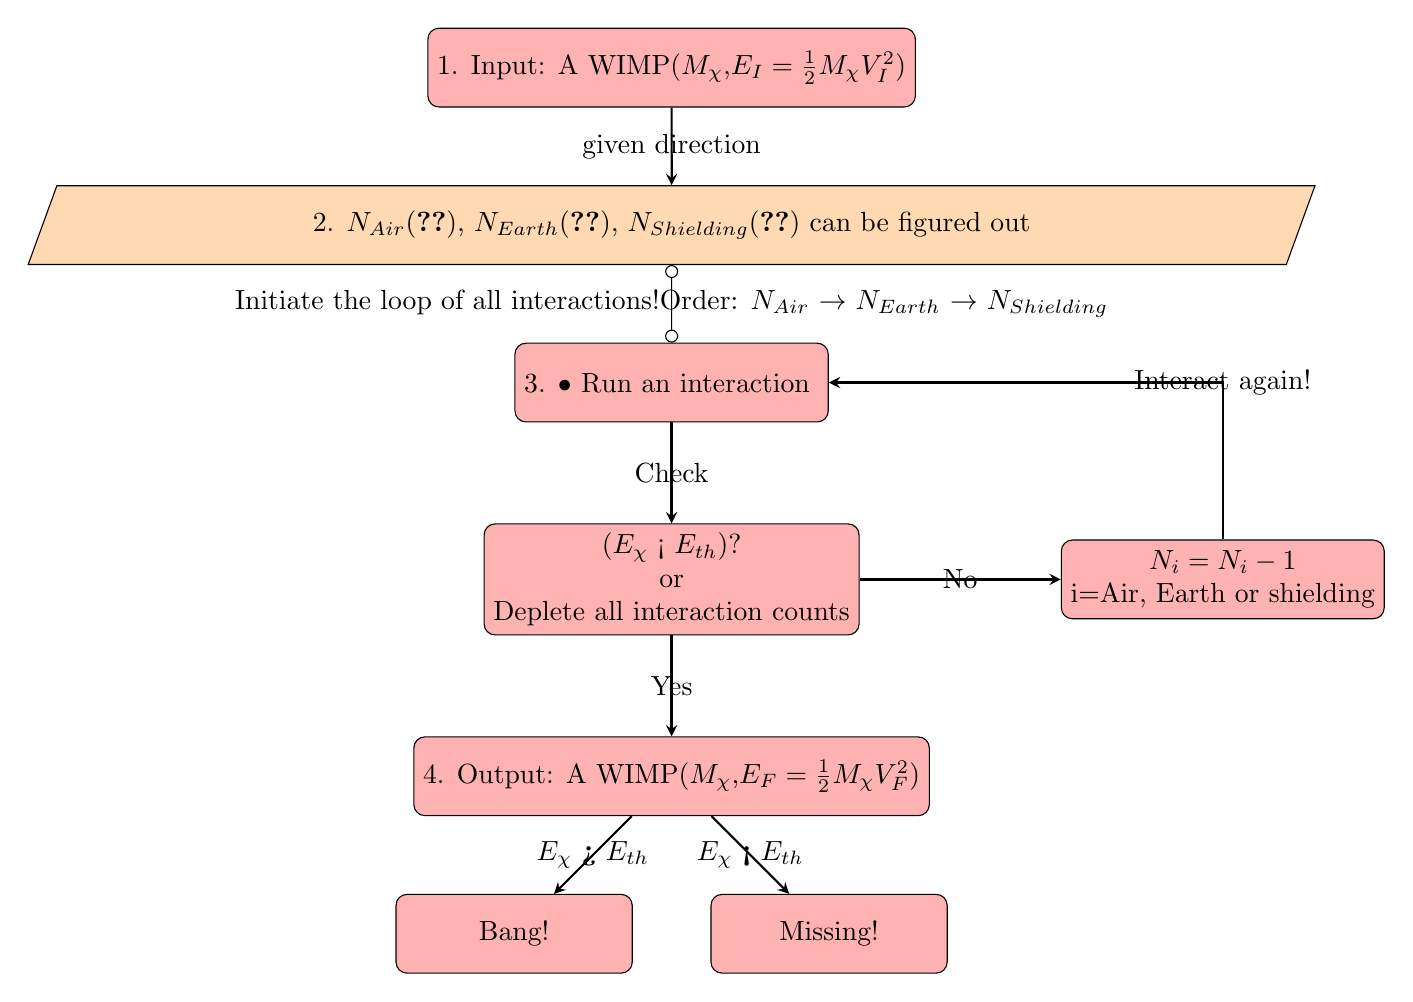
\begin{tikzpicture}[node distance=2cm]
\node (start) [startstop, align=center] {1. Input: A WIMP($M_{\chi}$,$E_{I}=\frac{1}{2}M_{\chi}V_{I}^{2}$)};
\node (in1) [io, below of=start, align=center] {2. $N_{Air}$(\ref{Earth_Interaction}), $N_{Earth}$(\ref{Air_Interaction}), $N_{Shielding}$(\ref{Shielding_Interaction}) can be figured out};
\node (Loop) [startstop, below of=in1, align=center] {3. $\bullet$ Run an interaction };
\node (endbf) [startstop, below of=Loop, align=center, yshift=-0.5cm] {($E_{\chi}$ < $E_{th}$)? \\ or \\ Deplete all interaction counts};

\node (endbf1) [startstop, right of= endbf, align=center, xshift=5cm] {$N_{i} = N_{i} - 1$ \\  i=Air, Earth or shielding};
\node (end) [startstop, below of=endbf, align=center, yshift=-0.5cm] {4. Output: A WIMP($M_{\chi}$,$E_{F}=\frac{1}{2}M_{\chi}V_{F}^{2}$)};

\node (Bang) [startstop, below of=end, align=center, xshift=-2cm] {Bang!};
\node (Missing) [startstop, below of=end, align=center, xshift=2cm] {Missing!};



\draw [arrow] (start) -- node{given direction}(in1);
\draw [o-o] (in1) -- node{Initiate the loop of all interactions! \\ Order: $N_{Air}$ $\rightarrow$ $N_{Earth}$ $\rightarrow$ $N_{Shielding}$}(Loop);
\draw [arrow] (Loop) -- node{Check}(endbf);
\draw [arrow] (endbf) -- node{No}(endbf1);
\draw [arrow] (endbf1) |- node{Interact again!}(Loop);
\draw [arrow] (endbf) -- node{Yes}(end);

\draw [arrow] (end) -- node{$E_{\chi}$ {\bf>} $E_{th}$}(Bang);
\draw [arrow] (end) -- node{$E_{\chi}$ {\bf<}  $E_{th}$}(Missing);

\end{tikzpicture}
\end{center}
\caption{The process of the count-based approach.} \label{Interaction_1}
\end{figure}

%%%%%%%%%%
\begin{comment}
\node (dec1) [decision, below of=pro1, yshift=-0.5cm] {Decision 1};
\node (pro2a) [process, below of=dec1, yshift=-0.5cm] {Process 2a};
\node (pro2b) [process, right of=dec1, xshift=2cm] {Process 2b};
\node (out1) [io, below of=pro2a] {Output};
\node (stop) [startstop, below of=out1] {Stop};
\end{comment}
\begin{comment}
\draw [arrow] (in1) -- (pro1);
\draw [arrow] (pro1) -- (dec1);
\draw [arrow] (dec1) -- node[anchor=east] {yes} (pro2a);
\draw [arrow] (dec1) -- node[anchor=south] {no} (pro2b);
\draw [arrow] (pro2b) |- (pro1);
\draw [arrow] (pro2a) -- (out1);
\draw [arrow] (out1) -- (stop);
\end{comment}
%%%%%%%%%%


\begin{enumerate}
	\item Generate a WIMP with a velocity based on the dark matter halo model and a random direction.\\
	\item Let it flee through the material of "solid earth, air and shielding" along a straight from our universe to the detector. Given the direction of the WIMP, the interaction counts in the different layers of three components can be estimated as follows:\\
	\begin{equation}
    \label{Interaction count}
    L \times D \times \sigma = N
    \end{equation}
    $L$ = The length a WIMP passes through the material\\
    $D$ = The density of the material that a WIMP passes through\\
    $\sigma$ = The total cross-section\\
    $N$ = The interaction count\\ 
	Since a variety of the densities in the different layers of solid earth, air and shielding should be regarded, the formulae for the aggregation of all compartments as follows:\\
	\begin{equation}
    \label{Earth_Interaction}
	\mathop{\sum_{i=1}^{18}} L_i \times D_i \times \sigma = N_{Air}
    \end{equation}
	\begin{equation}
    \label{Air_Interaction}
	\mathop{\sum_{i=1}^{18}} L_i \times D_i \times \sigma = N_{Earth}
    \end{equation}
	\begin{equation}
    \label{Shielding_Interaction}
	\mathop{\sum_{i=1}^{18}} L_i \times D_i \times \sigma = N_{Shielding}
    \end{equation}

	\item After reckoning the total counts for three components, the loop with the number of interactions can be launched. Run an interaction at a time. 
	  
	\item While the total count is depleted, or the energy of WIMP is smaller than the $E_{th}$, the velocity will be recorded soon and the process would be shut down.\\
\end{enumerate}

From this fashion, the merit of economizing time can be obtained as the count is the only parameter we should acquire, and let it enforce the loop of interactions directly till the energy of it is smaller than the threshold or attaining the detector. 

\section{Three-stage blockage for earth effect}
\subsection{Introduction to each stage}
Basically, the three-stage blocking effect can be foreseen as three components on the way WIMPs fly to our detector. All WIMPs could be blocked from reaching the detector at a certain stage, depending on the interaction counts.\\
\begin{enumerate}
\item Stage-1: No-effect stage\\
$\rightarrow$When the cross-section is too small to make a WIMP have an interaction with the atom, any material won't have an impact on the WIMPs, and they can freely pass through three components. 
\item Stage-2: Solid-earth-effect stage\\ 
$\rightarrow$Since the high densities of the solid earth with the long lengths that WIMPs pass by, the solid earth is the priority of involving interacting with the WIMPs. 
\item Stage-3: Shielding-and-air effect stage\\
$\rightarrow$At last, the shielding of the detector amalgamating with the air would entirely block all of the WIMPs from getting to the detector. 

\end{enumerate}

For the case of the TEXONO experiment, since it is being manipulated on the surface without the weighty shielding and heavy building nearby, most of the WIMPs could be still alive till the third stage. In another case, if you choose the extreme case, such as CDEX considered in our studies, all of the WIMPs could be blocked when transiting to the second stage as there is an extremely gigantic mountain covering its detector. By and large, It depends on the place where you set up for your detector and the structure of the environment, resulting in the disparage outcome for the upper limits of the cross-sections from a variety of the experiments located at the different positions. \\ 

\subsection{Velocity distributions}
Ahead of recognizing the spectrums for three interacting channels, which are used to set up limits for WIMPs, the velocity distributions for the different masses at the different cross-sections should be made out in the first place.\\ 

In Figure\ref{}, the velocity distributions with the gradually heightened cross-section are demonstrated with the count-based method at $M_{\chi}=10GeV$. The phenomenon, which is that the fewer and fewer event can be observed with the detectable energies with respect to the enhanced cross-sections, can be espied with the red lines in the figure.\\ 

The cardinal concept is that when the cross-section is getting larger, the interacting strength between the WIMP and the atom is getting stronger, implying the more energy transfusion of WIMP for every interaction with the material of solid earth, air, and shielding. After all, the energies of all WIMPs are weaker than the detector threshold, leading to the actuality that none of them can be detected by our detector. \\

\begin{figure}[]
\captionsetup[subfigure]{}
\centering

\subcaptionbox{(a)}{\includegraphics[width=0.4\columnwidth]{/Users/yehchihhsiang/Desktop/Analysis/CDEX_Analysis_method/Codes/Thesis_Plot/The_Basic_Flux/1_Used.pdf}}
\subcaptionbox{(b)}{\includegraphics[width=0.4\columnwidth]{/Users/yehchihhsiang/Desktop/Analysis/CDEX_Analysis_method/Codes/Thesis_Plot/The_Basic_Flux/1_Used.pdf}} 
\subcaptionbox{(a)}{\includegraphics[width=0.4\columnwidth]{/Users/yehchihhsiang/Desktop/Analysis/CDEX_Analysis_method/Codes/Thesis_Plot/The_Basic_Flux/1_Used.pdf}}
\subcaptionbox{(b)}{\includegraphics[width=0.4\columnwidth]{/Users/yehchihhsiang/Desktop/Analysis/CDEX_Analysis_method/Codes/Thesis_Plot/The_Basic_Flux/1_Used.pdf}} 
\subcaptionbox{(a)}{\includegraphics[width=0.4\columnwidth]{/Users/yehchihhsiang/Desktop/Analysis/CDEX_Analysis_method/Codes/Thesis_Plot/The_Basic_Flux/1_Used.pdf}}
\subcaptionbox{(b)}{\includegraphics[width=0.4\columnwidth]{/Users/yehchihhsiang/Desktop/Analysis/CDEX_Analysis_method/Codes/Thesis_Plot/The_Basic_Flux/1_Used.pdf}} 

\caption{The distributions of the velocity at 10GeV under the different cross-sections are shown. }\label{}
\end{figure}

\subsection{Recoil Spectrums}
In Figure\ref{}, Figure\ref{} and Figure\ref{}, they exhibit a series of the plots mirroring the
spectrums due to the Migdal Effect with regard to the cross-sections from the
the smaller one to the bigger one under the different stages. 
In Figure\ref{}, the no-effect stage is performed clearly with the evidence that two lines are overlapping together. 
In Figure\ref{}, the spectrums of the earth cases sluggishly lessen as the solid-earth-effect stage commence involving in. In the end, in Figure\ref{}, the spectrums of the earth effect cases dramatically drop when the cross-section is magnified, resulting in all of the WIMPs are blocked by the shielding and air, which is called the "shielding-and-air effect stage".

\begin{figure}[]
\captionsetup[subfigure]{}
\centering

\subcaptionbox{(a)}{\includegraphics[width=0.4\columnwidth]{/Users/yehchihhsiang/Desktop/Analysis/CDEX_Analysis_method/Codes/Thesis_Plot/Recoil_Spectrum/0P2GeV_MD_BR_1.pdf}}
\subcaptionbox{(b)}{\includegraphics[width=0.4\columnwidth]{/Users/yehchihhsiang/Desktop/Analysis/CDEX_Analysis_method/Codes/Thesis_Plot/Recoil_Spectrum/0P2GeV_MD_BR_2.pdf}} 
\subcaptionbox{(b)}{\includegraphics[width=0.4\columnwidth]{/Users/yehchihhsiang/Desktop/Analysis/CDEX_Analysis_method/Codes/Thesis_Plot/Recoil_Spectrum/0P2GeV_MD_BR_3.pdf}} 
\subcaptionbox{(b)}{\includegraphics[width=0.4\columnwidth]{/Users/yehchihhsiang/Desktop/Analysis/CDEX_Analysis_method/Codes/Thesis_Plot/Recoil_Spectrum/0P2GeV_MD_BR_4.pdf}} 
\subcaptionbox{(b)}{\includegraphics[width=0.4\columnwidth]{/Users/yehchihhsiang/Desktop/Analysis/CDEX_Analysis_method/Codes/Thesis_Plot/Recoil_Spectrum/0P2GeV_MD_BR_4.pdf}} 
\subcaptionbox{(b)}{\includegraphics[width=0.4\columnwidth]{/Users/yehchihhsiang/Desktop/Analysis/CDEX_Analysis_method/Codes/Thesis_Plot/Recoil_Spectrum/0P2GeV_MD_BR_4.pdf}} 

\caption{}\label{}
\end{figure}

\begin{figure}[]
\captionsetup[subfigure]{}
\centering

\subcaptionbox{(a)}{\includegraphics[width=0.4\columnwidth]{/Users/yehchihhsiang/Desktop/Analysis/CDEX_Analysis_method/Codes/Thesis_Plot/Recoil_Spectrum/0P2GeV_MD_BR_1.pdf}}
\subcaptionbox{(b)}{\includegraphics[width=0.4\columnwidth]{/Users/yehchihhsiang/Desktop/Analysis/CDEX_Analysis_method/Codes/Thesis_Plot/Recoil_Spectrum/0P2GeV_MD_BR_1.pdf}} 
\subcaptionbox{(b)}{\includegraphics[width=0.4\columnwidth]{/Users/yehchihhsiang/Desktop/Analysis/CDEX_Analysis_method/Codes/Thesis_Plot/Recoil_Spectrum/0P2GeV_MD_BR_1.pdf}} 
\subcaptionbox{(b)}{\includegraphics[width=0.4\columnwidth]{/Users/yehchihhsiang/Desktop/Analysis/CDEX_Analysis_method/Codes/Thesis_Plot/Recoil_Spectrum/0P2GeV_MD_BR_1.pdf}} 

\caption{}\label{}
\end{figure}

\begin{figure}[]
\captionsetup[subfigure]{}
\centering

\subcaptionbox{(a)}{\includegraphics[width=0.4\columnwidth]{/Users/yehchihhsiang/Desktop/Analysis/CDEX_Analysis_method/Codes/Thesis_Plot/Recoil_Spectrum/0P2GeV_MD_BR_1.pdf}}
\subcaptionbox{(b)}{\includegraphics[width=0.4\columnwidth]{/Users/yehchihhsiang/Desktop/Analysis/CDEX_Analysis_method/Codes/Thesis_Plot/Recoil_Spectrum/0P2GeV_MD_BR_1.pdf}} 
\subcaptionbox{(b)}{\includegraphics[width=0.4\columnwidth]{/Users/yehchihhsiang/Desktop/Analysis/CDEX_Analysis_method/Codes/Thesis_Plot/Recoil_Spectrum/0P2GeV_MD_BR_1.pdf}} 
\subcaptionbox{(b)}{\includegraphics[width=0.4\columnwidth]{/Users/yehchihhsiang/Desktop/Analysis/CDEX_Analysis_method/Codes/Thesis_Plot/Recoil_Spectrum/0P2GeV_MD_BR_1.pdf}} 

\caption{}\label{}
\end{figure}

\subsection{Sensitivity Line for Quantifying the earth effect}
Since the spectrums from the different channels are already expressed in the previous section, how to quantify the effects for different stages should be addressed. In the following formula, the ratio of survival flux to the original flux, can be adopted to do the quantification:\\
 	\begin{equation}
        \label{Interaction count modification}
	\sigma_{\text{SI}}^{\text{Sensitivity}} = \sigma_{\text{SI}}^{\text{real}}  \times \frac{ \text{Survival Flux}}{\text{Original Flux}}
        \end{equation}
As the cross-section is getting higher, the survival flux will become lower, at certain point, the ratio of that will be zero, which means there is no WIMP that can be detected. There are two examples, which are derived from two experiments, demonstrated at $M_{\chi}$ = 10GeV as follows.\\ 

In figure\ref{}, the sensitivity line for CDEX is shown. The clear pattern is shown that when the cross-section is very small, the flux won't be affected by the earth as the description in stage-1. As the cross-section is getting higher, it alters into the stage-2 , which indicates that the interaction between the atoms of earth and WIMPs initiates. In the end, all of the WIMPs will be hampered by the mountain, which is held accountable for consuming all WIMPs.\\ 

Differing from the underground experiment as CDEX, TEXONO experiment on the surface can accepts more amount of WIMPs having the detector-triggering energy when being under the same cross-section. In Figure\ref{}, the lower $\sigma_{SI}$ that can achieved is expected as there is no other gigantic objects mounted nearby the detector, and all of WIMPs will be impeded by the shielding and building as its transformation into the stage-3.
 
        \begin{figure}[h]
        \includegraphics[scale=0.6]{/Users/yehchihhsiang/Desktop/Analysis/CDEX_Analysis_method/Codes/Thesis_Plot/Sensitivity_Line/KS_Line.pdf}
        \centering
        \caption{} \label{Vacuum-constrained WIMPs}
        \end{figure}

         \begin{figure}[h]
        \includegraphics[scale=0.6]{/Users/yehchihhsiang/Desktop/Analysis/CDEX_Analysis_method/Codes/Thesis_Plot/Sensitivity_Line/CDEX_Line.pdf}
        \centering
        \caption{} \label{Vacuum-constrained WIMPs}
        \end{figure}

\section{Earth-constrained limits on WIMPs}
In the end, earth-constrained limits on WIMPs should be brought out for two experiments. As the sensitivity lines are worked out in the previous sections, the vacuum-constrained limits can be added to the plots for acquiring the corresponding $\sigma_{SI}$ for both upper boundary and lower boundary.\\

In Figure\ref{}, the limit-setting standard plot is expressed with the Migdal effect channel at TEXONO. After the earth-constrained line is completed, which is described in the previous, the  
vacuum-constrained limit can be overlapped together with that. Then, the $\sigma_{SI}$ for the boundaries are crystal clear. 
         \begin{figure}[h]
        \includegraphics[scale=0.6]{/Users/yehchihhsiang/Desktop/Analysis/CDEX_Analysis_method/Codes/Thesis_Plot/Sensitivity_Line/KS_Line_overlap.pdf}
        \centering
        \caption{} \label{Vacuum-constrained WIMPs}
        \end{figure}
        
In finale, the territory on the map of $\sigma_{SI}$ and $M_{\chi}$, which is called "exclusion plot",  based on the capability of exploring the WIMP should be rolled out for the comparisons between different experiments. the bigger the territory that experiment can claim, the higher the possibility of discovering the WIMP they have.\\

As the upper and lower boundaries clarified by the red lines in Figure\ref{} for Migdal effect at $M_{\chi}$=0.8GeV, the boundaries for the rest of the masses can be completed with the same process demonstrated (shown in the appendix) and the enclosed territory can be drafted.\\

To compare with the territories claimed by other experiments working on unveiling WIMP mystery, the territory taken over by our buildup should be overlapped with others in the same plot. Figure\ref{} illustrates the exclusion plot for CDEX with the Migdal effect. In accordance with the sensitivity lines for Brem at CDEX, since the vacuum-constrained $\sigma_{SI}$ is too high to cross the earth-constrained line as an example in Figure\ref{}, leading to the tragedy of losing all of the chances to measure the WIMPs from sub-GeV to GeV mass with Brem channel.

\section{Conclusion}
In conclusion, first the capabilities of our experiments at CDEX and TEXONO on claiming 



%% This is an example first chapter.  You should put chapter/appendix that you
%% write into a separate file, and add a line \include{yourfilename} to
%% main.tex, where `yourfilename.tex' is the name of the chapter/appendix file.
%% You can process specific files by typing their names in at the 
%% \files=
%% prompt when you run the file main.tex through LaTeX. 
% MBA, CBA
\chapter{Method-\rom{2}: Movement-based Approach on Constraint for WIMP}
After exploring the first limits on WIMPs with Method-\rom{1}, the systematic error should be explored with Method-\rom{2}, considering the almost-authentic system. In this analysis, two cases are taken into account. The first one is the straight-line case, which is actually similar to our Method-\rom{1} but this time the 

\section{Introduction to the method}

Instead of the implantation of the interaction counts as being applied in the previous section, the movement-based approach, which suggests the step-by-step movement-and-interaction action, is revealing the genuine physical process. It shifts with a tiny length at a time, and rolls a dice to see if it would interact with the atom or not, in accordance with the Possion distribution. The method bewritted in this section is probed as the way to check the systematic difference compared with the count-based approach.\\

\begin{figure}
\begin{center}
\begin{tikzpicture}[node distance=2cm]
\node (start) [startstop, align=center] {Input: A WIMP($M_{\chi}$,$E_{I}=\frac{1}{2}M_{\chi}V_{I}^{2}$)};
\node (Length) [startstop, below of=start, align=center] {Move a distance given by the formula\ref{Interaction count modification}.  };

\node (Dice) [startstop, below of=Length, align=center] {Roll a dice!};

\node (Yes) [startstop, below of=Dice, align=center, xshift=-2cm] {Yes};
\node (No) [startstop, below of=Dice, align=center, xshift=2cm] {No};

\node (AnInteraction) [startstop, below of=Yes, align=center] {$\bullet$Run an interaction \\ A. With the scattering angle \\ B. Without the scattering angle};

\node (endbf) [startstop, below of=AnInteraction, align=center, xshift=2cm, yshift=-2cm] {(The energy of WIMP < $E_{th}$])? \\ or \\ (Reach the detector)? };

\node (rightofendbf) [startstop, right of=endbf, align=center, xshift=5cm]{Keep going on!};

\node (end) [startstop, below of=endbf, align=center, yshift=-0.5cm] {Output: A WIMP($M_{\chi}$,$E_{F}=\frac{1}{2}M_{\chi}V_{F}^{2}$)};

\node (Bang) [startstop, below of=end, align=center, xshift=-2cm] {Bang!};
\node (Missing) [startstop, below of=end, align=center, xshift=2cm] {Missing!};

\draw [o-o] (start) -- node{Start from the outmost layer of air}(in1);
\draw [arrow] (in1) -- node{}(Loop);

\draw [arrow] (Dice) -- node{1}(Yes);
\draw [arrow] (Dice) -- node{0}(No);
\draw [arrow] (Yes) -- node{}(AnInteraction);
\draw [arrow] (AnInteraction) -- node{Check}(endbf);
\draw [arrow] (No) -- node[yshift=-1.2cm]{Check}(endbf);

\draw [arrow] (endbf) -- node{No}(rightofendbf);
\draw [arrow] (rightofendbf) |- node{}(Length);
\draw [arrow] (endbf) -- node{Yes}(end);
\draw [arrow] (end) -- node{$E_{\chi}$ {\bf>} $E_{th}$}(Bang);
\draw [arrow] (end) -- node{$E_{\chi}$ {\bf<}  $E_{th}$}(Missing);

\end{tikzpicture}
\end{center}
\caption{The process of the movement-based approach.} \label{Interaction_1}
\end{figure}

\begin{enumerate}
	\item Generate a WIMP with a velocity based on the dark matter halo model and a random direction.\\
	\item With the formula\ref{Interaction count modification}, which is the same as \ref{Interaction count} but a slight movement, we can get the length that a WIMP goes through for the next step:\\
	\begin{equation}
        \label{Interaction count modification}
	L = \frac{N}{D \times \sigma}
        \end{equation}
        $L$ = The length a WIMP passes through the material\\
        $D$ = The density of the material that a WIMP passes through\\
        $\sigma$ = The total cross-section\\
        $N$ = The interaction count\\ 
	\item Since the interaction over two times for an interaction is impossible, a dice should be rolled with the Possion distribution which the $\lambda$ is 0.001 to see whether it will interact with the atom or nor. After every interaction, there are two cases:\\
	\begin{enumerate}
		\item Without the scattering angle:\\
		The WIMP continues running straightforward without any consideration.\\
		\item With the scattering angle:\\
		Derived from the two-dimensional collision, the following formula can be found in \ref{}:
		\begin{equation}
                 \label{Interaction count modification}
    		tan(\theta_{lab}) = \frac{sin(\theta_{rest})}{cos(\theta_{rest})+\frac{M1}{M2}}
                 \end{equation}
		M1 is the mass of the WIMP, M2 is the mass of the atom. $\theta$ is randomly chosen between 0 to 180 degree. After the final velocity of the WIMP as well as the scattering angle are determined, the direction of it can be decided as well.\\
	\end{enumerate} 
	\item Loop between 2. to 4. till the WIMP reaches the detector or the energy of it is smaller than the threshold.\\
\end{enumerate}

\section{Two-case movement}
To compare between these two methods for estimating the systematic error for method1, the sensitivity lines originating from these two methods would be overlapped to see the difference. In the following sections, two cases, including the straight trajectory as well as the bending trajectory, are competed to see.
\subsection{S-mode case}
The same as the count-based movement, the case here is using S-mode as the assumption to be the trajectory for WIMPs. In this case, the first thing that should be answered is: With the intuitive way of step-by-step movement, what happens to our final results on setting limits for WIMPs? Is there a significant difference between these two methods?\\

In Fig.\ref{}, the plot shows the pretty clear pattern that under this mode with the movement-based method, there is no significant difference from the count-based method. From the theoretical point, actually the expectation value is very close to the count-based values, so the similar results are envisioned.

\begin{figure}[]
\captionsetup[subfigure]{}
\centering

\subcaptionbox{(a)}{\includegraphics[width=0.4\columnwidth]{/Users/yehchihhsiang/Desktop/Analysis/CDEX_Analysis_method/Codes/Thesis_Plot/Sensitivity_Line/All_0P2GeV_STS_TEXONO_BR.pdf}}
\subcaptionbox{(b)}{\includegraphics[width=0.4\columnwidth]{/Users/yehchihhsiang/Desktop/Analysis/CDEX_Analysis_method/Codes/Thesis_Plot/Sensitivity_Line/All_20GeV_STS_TEXONO_NU.pdf}} 

\caption{}\label{}
\end{figure}

\subsection{B-mode case}
In finale, as the WIMPs pass through the material, they could be scattered with the atoms and derail to other directions, and possibly, some of them could pass longer length, along with accompanying more interaction counts before they arrive at the detector. Even more, some of them could be bent off the original direction extremely that they can't reach the detector. In this study, the bending case having the impact on setting limits for WIMPs is explored.\\ 

In this case, there is a slight difference compared with the previous studies. In order to make the studies more simpler, the CRESST case, which is one of the surface experiments, is simulated for the systematic error. Being distinct from the S-mode, which forces WIMPs to fly to the detector directly with a straight line, the method here is to let it freely move with the scattering processes till they attain the surface of the earth.\\ 

\begin{equation}
\label{Interaction count modification}
L_{B/S} = \frac{ \text{The B-mode path length}}{\text{The S-mode path length}} = \frac{L_{B}}{L_{S}}
\end{equation}

In Fig.\ref{}, the comparison between two cases, including S-mode and B-mode, is shown. Overall, the goal from this study is to find out the biggest systematic error and mark them for our study, so the thing that should be done here is to find out the biggest difference between these two sensitivity lines. As the studies done in the previous section, the boundaries for setting limits mostly emerge in the stage2(lower boundary) and stage3(upper boundary), the representative lines for these two stages from two modes are depicted to define our systematic error. Comparing between these two modes, some of the intriguing issue can be made as follows:

\begin{enumerate}
\item  Stage2:\\
There is a clear tendency that can be observed is that, when the mass becomes smaller and smaller, the red line, meaning the B-mode case, is getting lefter, closing to the vacuum-constrained line. The proof of this is in Fig.\ref{}, it shows the ratio of the B-mode path length to the S-mode path length. When the mass of WIMP is getting lower, it could be bent dramatically when it gets to the earth, and quickly return back to the surface, leading to the smaller ratio as seen in figure. The smaller the ratio, the higher the energy that would be preserved by WIMPs, resulting in the near vacuum-like case. 
\item  Stage3:\\
The opposite case happens to the stage3, compared with the stage2. As the mass grows lower, the WIMPs should pass more longer case to arrive at the detector, furthermore, some of them could be off the road to the surface. As a result, when the mass is getting lower, the red line becomes more lefter. The Fig\ref{} proves our point of view that the higher mass corresponds to the higher $L_{B/S}$, 
\end{enumerate}

\begin{figure}[]
\captionsetup[subfigure]{}
\centering

\subcaptionbox{(a)}{\includegraphics[width=0.4\columnwidth]{/Users/yehchihhsiang/Desktop/Analysis/CDEX_Analysis_method/Codes/Thesis_Plot/Sensitivity_Line/All_20GeV_STS_Bent.pdf}}
\subcaptionbox{(b)}{\includegraphics[width=0.4\columnwidth]{/Users/yehchihhsiang/Desktop/Analysis/CDEX_Analysis_method/Codes/Thesis_Plot/Sensitivity_Line/All_2GeV_STS_Bent.pdf}} 
\subcaptionbox{(b)}{\includegraphics[width=0.4\columnwidth]{/Users/yehchihhsiang/Desktop/Analysis/CDEX_Analysis_method/Codes/Thesis_Plot/Sensitivity_Line/All_0P2GeV_STS_Bent.pdf}} 

\caption{}\label{}
\end{figure}



%% This is an example first chapter.  You should put chapter/appendix that you
%% write into a separate file, and add a line \include{yourfilename} to
%% main.tex, where `yourfilename.tex' is the name of the chapter/appendix file.
%% You can process specific files by typing their names in at the 
%% \files=
%% prompt when you run the file main.tex through LaTeX.
\chapter{Conclusion for Our Analysis}

\chapter{Extension:Low-threshold detector development}

\begin{comment}
\section{\label{sec:level1}Introduction:\protect\\
Why GeIA? and The issue}

For the exploration of the lower-mass region for WIMPs, the first immediate idea is "Since the signal of WIMP is so small, why don't we just amplify it?" Some people commenced their contemplation on the technical works.\\

In 2000, two smart Russian guys came up with the brilliant idea about applying the high voltage on the Ge detector, and the signal will be amplified by the avalanche region emerging in the crystal under the high voltage. Now, there are a bunch of experiments trying to extend the idea and to see whether it can be worked out with the more state-of-the-art technique.\\ 

Although the internal amplification seems a good idea, the noise of the crystal could be unexpectedly amplified as well. Dealing with the issue of the high noise originating from the leakage current is another topic for this experiment. In this document, we will also confirm the issue of the noise in the crystal.\\

In our collaborations, we have two teams working on the idea under two conventional temperatures, which are 4K(USD) and 77K(THU). I would like to explore that under these two temperatures, what will happen to the crystal from the perspective of "the signal" and also "the noise" under the high voltage.


%%%%%%%%%%%%%%%%%%%%%%%%%%%%%%%%%%%%%%%%%%%%%%%%%%%%%%%%

\section{\label{sec:level2}Basic p-n junction}
Given the semiconductor containing the different types of impurity, we can get two groups, including the n(electron-dominant) and p(hole-dominant) types. For any crystal containing both types of semiconductors, the properties of the p-n junction will occur by and large. I would like to briefly discuss the phenomenon for it.\\

On the p-n junction, the electron-hole diffusion, as well as the attraction, will start emerging in the crystal. After the "dynamic" get balance, the neutral region called "the depletion region" that the stable electric field flows in will show up. In the reverse-bias case, the higher the voltage, the bigger the region it will be. In the end, we need to increase the voltage to the one which can deplete all the crystal, meaning that all electrons and holes in the crystal get balance. Then, we can start our usage of the crystal.\\

If you want to know more details about the fundamental physics in semiconductor, I recommend the book\cite{10.5555/1594006}, chapter7 and chapter8, or wiki page.

%%%%%%%%%%%%%%%%%%%%%%%%%%%%%%%%%%%%%%%%%%%%%%%%%%%%%%%%

\section{\label{sec:level3}signal amplification}

\subsection{From the perspective of "an electron":}
At the start, let us imagine "an electron", which is ionized by a WIMP,  flowing in the crystal. There are many important parameters that we should acquire from it for opening our studies. I will depict them in the following paragraph.

\begin{enumerate}
	\item Electrical Mobility($\mu$): Related to the conductivity of the electron in the crystal. In the paper\cite{7}, basically, all of the important information is included. From the formula2 of paper\cite{7}, which is used to summarize the mobility, we can see that the smaller the individual mobility, the higher the importance that is. From our research, actually, the acoustic phonon scattering is the dominant term for 77K, and the neutral impurity scattering, which is not affected by the temperature normally, is the dominant term for 4K. You can compare between Fig.2 and Fig.3 in the paper\cite{7}.
	\item Effective mass(m*): Under the different temperatures, the conductivity effective masses are various. Fig.5. of the paper\cite{6} describes the effective mass with respect to the temperature. Since there is no such study for Ge, we just take Si as our standard in this case to give us a sense on the tendency of it.
	\item Relaxation Time($\tau$): The period of time that the electron can run without bumping into another atom. You can also find out the formula in the paper\cite{7}.
	
	\begin{equation}
    \tau = \frac{\mu \times m*}{e}
    \end{equation}
	e is the coulomb constant\\
	
	After acknowledging the relaxation time, the next thing we need to figure out is the mean free path($\L$). which means how far the electron can go without colliding with another atom in the crystal. The formula is as follows:
\begin{equation}
\label{MFP}
L = \tau \times V_{d}
\end{equation}
$V_{d}$ means the velocity of the electron. 
	\item electron velocity($V_{d}$): The relation between the velocity of the electron and the voltage applied to the crystal is demonstrated in Fig.1 of the paper\cite{5}. 
\end{enumerate}

After all of the parameters are well-recognized in this section, we will use some of them in the next section and start our journey on the amplification. 




\subsection{Ionization rate}
The definition of ionization rate: How many electrons/holes can be ionized within 1cm?\\

After depleting the crystal, next we would like to ask the relation between the ionization rate and the E(V/cm). Based on the formula(20a) in \cite{2}, which can determine the ionization rate by figuring out mean free path(L), electric field(E(x)) and ionization energy(U) of the material, we can get FIG.\ref{fig1}. There are three important pieces of information given by this:\\

\begin{figure}[h]
  \centering
  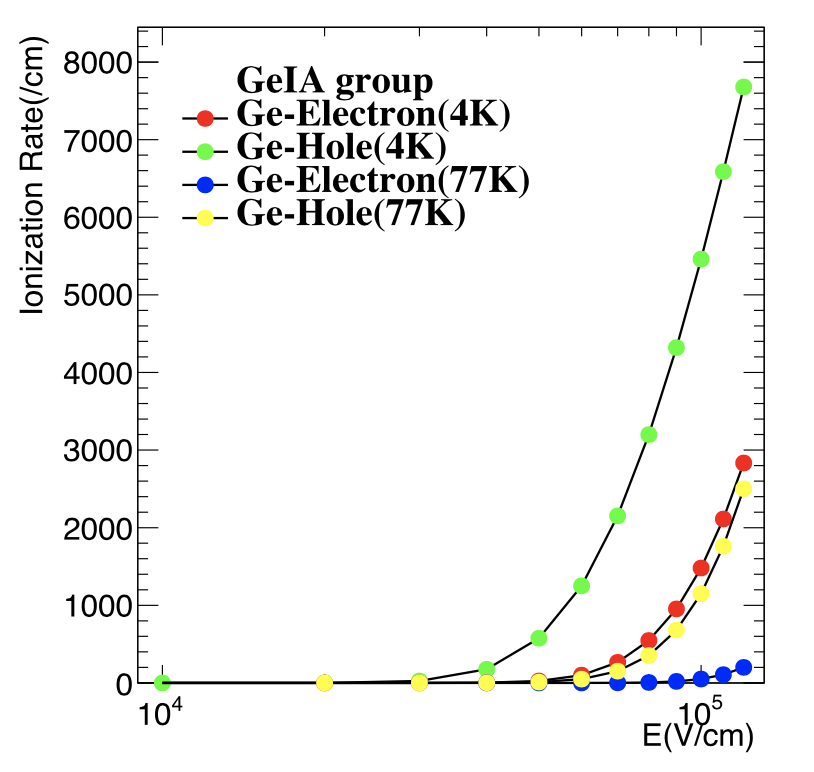
\includegraphics[width=0.35\textwidth]{SHEME/Ionization_rate.png}
  \caption{The ionization rates for both electron and hole under both 4K and 77K.}
  \label{fig1}
\end{figure}

\begin{enumerate}
	\item Critical E=$10^{4}$ V/cm
	\item The significant difference between e/h cases is the effective mass under such high electric field at the same T.
	\item Hole can give us more signal under the lower T.
\end{enumerate}

\subsection{Pioneer: Russian investigation[2000]}
In light of the paper\cite{1}, the conceptual design on the coaxial detector HPGe with the impurity of the crystal is provided. The key point is as the following sentence.\\ 

According to FIG.\ref{fig1}, when the electric field is higher than $10^{4}$(V/cm), the electron will be increased as the function of the electric field. Because of that, there are two regions that can be marked in FIG.2, given by Fig. 1 of the paper\cite{1}:

\begin{figure}[h]
  \centering
  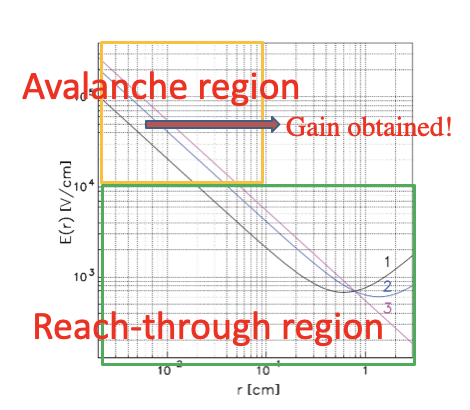
\includegraphics[width=0.35\textwidth]{SHEME/Avalanche_Reach_Through.png}
  \caption{The electric field as a function of the distance from the strip with the different impurities. The number above the lines mean the different impurities: (1)$10^{10} cm^{-3}$, (2)4 $\times 10^{9} cm^{-3}$ and (3) 0 $cm^{-3}$}
  \label{fig2}
\end{figure}

\begin{enumerate}
	\item Avalanche region: When the electric field is above $10^{4}$(V/cm), the avalanche effect will emerge, and the signal will be amplified. 
	\item Reach-through region: Below that, since the electron/hole will just go through normally without any effect on them.
\end{enumerate}

These studies give us a clue that we can devise a detector that can produce the amplification for the signal with the electric field above a certain level.
%%%%%%%%%%%%%%%%%%%%%%%%%%%%%%%%%%%%%%%%%%%%%%%%%%%%%%%%

\section{\label{sec:level3}noise in the crystal}
Unfortunately, the noise in the crystal is inevitable. The genres of the noise in the crystal should be characterized as the criteria of acquiring the feasibility of measuring dark matter theoretically. 
There are three kinds of noise in the crystal, encompassing the bulk leakage current, the contact leakage current, and the surface leakage current. In the following paragraph, I will depict them individually.\\

\subsection{Bulk leakage current}
Because of the thermal fluctuation, the electrons from the bulk(purity, such as Ge) material will be ionized possibly. Fortunately, the level of this noise can be ignored below 77K. The associated information is well-written in the formula(6) of paper\cite{doi:10.1063/1.4953147}. We can use the formula as follows to estimate the current.
\begin{equation}
I = A e^{\frac{-E_{Ge Band}}{2k_{B}T}}*q
\end{equation}
A=intrinsic concentration, $E_{Ge Band}$=Ge bandgap, q=coulomb constant, T= temperature(K)
\subsection{Contact leakage current}
Because of 
\begin{enumerate}
	\item The barrier between the semi-metal connection
	\item The thermal fluctuation
\end{enumerate}
There is a possibility that the electron in the conductive band of the semiconductor could jump into the metal, leading to the dark current which is unwanted. Fig.8 of the paper\cite{LOOKER2015138} and Fig. 10 of the paper\cite{Wei_2018} perform the leakage current at the different temperatures. The current at a certain temperature can be predicted by these two figures. \\

The fundamental physics is "Schottky effect", which is a kind of the thermal emission. We can express the simplified formula with the "Richardson's law" as follows: 
\begin{equation}
I \propto T^{2} e^{\frac{W}{k_{B}T}}
\end{equation}
$E_{Ge Band}$=Ge band gap q=coulomb constant 
T= temperature(K), W= work function of the material, A=Measured constant\\

You can find out the detail in the book\cite{10.5555/1203347}. This leakage current will be the dominant one under 77K.\\

Basically, it is a Metal-Semiconductor junction problem, which is a very big topic authentically and you can see the chapter 10, 11 of book\cite{10.5555/1203347}(Strongly recommended!) and chapter 6 and 7 of book\cite{MILNES1972171} for more detail.\\

\subsection{Surface leakage current}
It depends on the quality of the crystal. Although lowering the temperature will help decrease the noise, the mechanism of this current is not clear for now. We can only rely on the measurement.\\ 

There is a paper on measuring the surface leakage current for the semiconductor. Please look at Fig.2 of the paper\cite{5871995}. You can extend the points in the figure to predict the surface leakage current. Although it is not for Ge, it can give us a hint on the scale of the surface leakage current for semiconductors. This leakage current will be the dominant one under 4K.


\section{Conclusion and dilemma}

\begin{enumerate}
	\item If we can suppress the surface leakage current, we can get the lower threshold detector. But unfortunately, now there is no good way to decrease it. 
	\item Under the high temperature, such as 77K, the crystal could easily break down because of the high leakage current, now we would like to start with the experiment under 4K to produce a first version stable amplification. 
\end{enumerate}


\bibliographystyle{apsrev4-2} % Tell bibtex which bibliography style to use
\bibliography{GeIANotes_Used}
\end{comment}





\appendix
\chapter{Tables}

\begin{table}
\caption{Armadillos}
\label{arm:table}
\begin{center}
\begin{tabular}{||l|l||}\hline
Armadillos & are \\\hline
our	   & friends \\\hline
\end{tabular}
\end{center}
\end{table}

\clearpage
\newpage

\chapter{Figures}

\vspace*{-3in}

\begin{figure}
\vspace{2.4in}
\caption{Armadillo slaying lawyer.}
\label{arm:fig1}
\end{figure}
\clearpage
\newpage

\begin{figure}
\vspace{2.4in}
\caption{Armadillo eradicating national debt.}
\label{arm:fig2}
\end{figure}
\clearpage
\newpage

%% This defines the bibliography file (main.bib) and the bibliography style.
%% If you want to create a bibliography file by hand, change the contents of
%% this file to a `thebibliography' environment.  For more information 
%% see section 4.3 of the LaTeX manual.
\begin{singlespace}
\bibliography{main}
\bibliographystyle{plain}
\end{singlespace}

\end{document}

